\documentclass[hidelinks]{ctexart}

\usepackage{van-de-la-illinoise}
\usepackage[paper=b5paper,top=.3in,left=.9in,right=.9in,bottom=.3in]{geometry}
\usepackage{calc}
\pagenumbering{gobble}
\setlength{\parindent}{0pt}
\sisetup{inter-unit-product=\ensuremath{{}\cdot{}}}

\newdimen\indexlen
\def\newprobheader#1{%
\def\probindex{#1}
\setlength\indexlen{\widthof{\textbf{\probindex}}}
\hskip\dimexpr-\indexlen-1em\relax
\textbf{\probindex}\hskip1em\relax
}
\def\newprob#1{%
\newprobheader{#1}%
\def\newprob##1{%
\probsep%
\newprobheader{##1}%
}%
}
\def\probsep{\vskip1em\relax{\color{gray}\dotfill}\vskip1em\relax}

\begin{document}

\newprob{3.9 (1)}%
\\[-2.5\baselineskip]
\begin{center}
    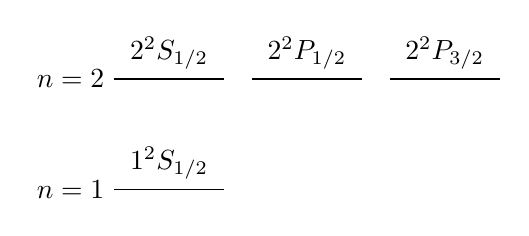
\begin{tikzpicture}[scale=0.7]
        \draw (0,0) node[left] {$n=1$} -- (2,0)
        (1,0) node[above] {$\ce{1^2S_{1/2}}$}
        (0,2) node[left] {$n=2$} -- (2,2)
        (1,2) node[above] {$\ce{2^2S_{1/2}}$}
        (2.5,2) -- (4.5,2)
        (3.5,2) node[above] {$\ce{2^2P_{1/2}}$}
        (5,2) -- (7,2)
        (6,2) node[above] {$\ce{2^2P_{3/2}}$};
    \end{tikzpicture}
\end{center}
\par
\newprobheader{(2)}%
$n=1$: 相对论效应, Lamb移位, 超精细结构.\\
$n=2,\ l=0$: 相对论效应, Lamb移位, 超精细结构.\\
$n=2,\ l=1$: 自旋-轨道耦合, 相对论效应, Lamb移位, 超精细结构.\\
自旋-轨道耦合$\sim$相对论效应$>$Lamb移位$>$超精细结构.
\newprob{I}%
\\[-3.25\baselineskip]
\begin{center}
    \begin{tabular}{ccccc}
        轨道 & 精细结构 & Lamb移位 & 总修正 & 减去基态 \\
        & $\scriptstyle -E_n \frac{\alpha^2}{n^2}(\frac{3}{4} - \frac{n}{j+1/2})$ & $\scriptstyle  \frac{m_ec^2\alpha^4}{2n^3}\times 0.0485$ & \\
        $\ce{2^2P_{3/2}}$ & $\SI{-1.13e-5}{\eV}$ & & $\SI{-1.13e-5}{\eV}$ & $\SI{13.5e-5}{\eV}$ \\
        $\ce{2^2S_{1/2}}$ & $\SI{-5.66e-5}{\eV}$ & $\displaystyle \SI{0.439e-5}{\eV} $ & $\SI{-5.22e-5}{\eV}$ \\
        $\ce{2^2P_{1/2}}$ & $\SI{-5.66e-5}{\eV}$ & & $\SI{-5.66e-5}{\eV}$ & $\SI{8.94e-5}{\eV}$ \\
        $\ce{1^2S_{1/2}}$ & $\SI{-18.1e-5}{\eV}$ & $\displaystyle \SI{3.51e-5}{\eV} $ & $\SI{-14.6e-5}{\eV}$ \\
    \end{tabular}
\end{center}
$\ce{2^2P_{3/2}}\mapsto \ce{1^2S_{1/2}}$: $\displaystyle \frac{\Delta E}{E} = 1.32\times 10^{-5}$. 波长$\displaystyle \frac{1/\pare{1+1.32\times 10^{-5}}}{\displaystyle R_H\pare{1-\rec{4}}} = \boxed{\SI{1215.668}{\angstrom}.}$ \\
$\ce{2^2P_{1/2}}\mapsto \ce{1^2S_{1/2}}$: $\displaystyle \frac{\Delta E}{E} = 0.876\times 10^{-5}$. 波长$\displaystyle \frac{1/\pare{1+0.876\times 10^{-5}}}{\displaystyle R_H\pare{1-\rec{4}}} = \boxed{\SI{1215.674}{\angstrom}.}$ \\
分裂为两条, 间隔约$\SI{0.006}{\angstrom}$.
\newprob{II}%
$j = 1/2$, $I = 1/2$, $F = 1,0$. 故
\begin{align*}
    & \Delta E = \frac{a}{2}\brac{F\pare{F+1} - J\pare{J+1} - I\pare{I+1}} = \curb{\rec{4}a,-\frac{3}{4}a}\\ & \Rightarrow \Delta = a = h\nu = \boxed{\SI{5.87e-6}{\eV}.}
\end{align*}
\newprob{III}%
$\displaystyle a = -2g\+_s_\pare{\frac{m_e}{m_e}}\frac{\alpha^2 Z}{n}E_n \rec{j\pare{j+1}\pare{2l+1}}$. 取$g\+_s_=2$, $n=1$, $j=1/2$, $l=0$, $\displaystyle E_n = -\half \times \SI{13.6}{\eV} = -\SI{6.8}{\eV}$ $\Rightarrow \Delta = a = \boxed{\SI{1.93e-3}{\eV}.}$
\newprob{3.10 (1)}%
$\ce{7s}\mapsto \ce{6p}$, 由$\ce{6p}$劈裂为\underline{$\ce{6 ^2P_{1/2}}$, $\ce{6 ^2P_{3/2}}$}引起.
\par
\newprobheader{(2)}%
$\displaystyle \Delta E = hc\abs{\tilde{\nu}_1 - \tilde{\nu}_2} = \boxed{\SI{0.0687}{\eV}.}$
\par
\newprobheader{(3)}%
$\displaystyle \Delta E = \half g_s \pare{m_s - m_s'}\mu\+_B_\cdot B$, 其中最开始的$1/2$因子由Thomas旋进贡献, 故$B = \boxed{\SI{1186}{\tesla}.}$
\newprob{3.11 (1)}%
\\[-2\baselineskip]
\begin{center}
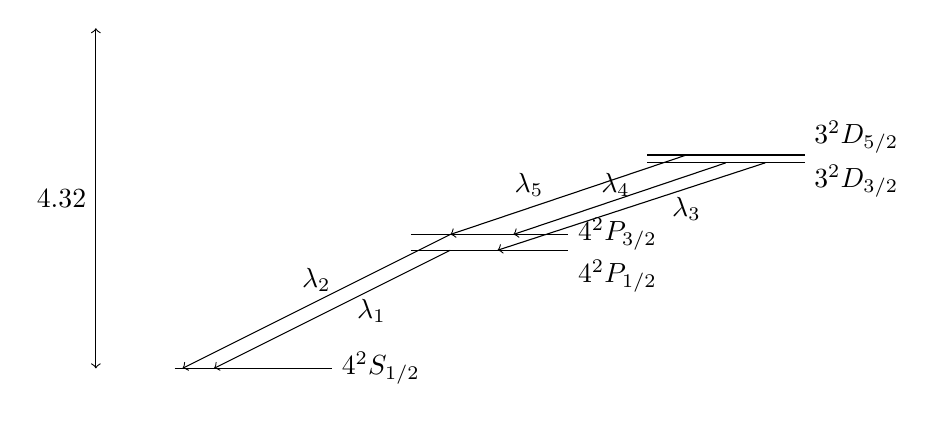
\begin{tikzpicture}
    \draw (0,0) -- (2,0) node [right] {$\ce{4 ^2S_{1/2}}$}
        (3,1.5) -- (5,1.5) node [below right] {$\ce{4 ^2P_{1/2}}$}
        (3,1.7) -- (5,1.7) node [right] {$\ce{4 ^2P_{3/2}}$}
        (6,2.71) -- (8,2.71) node [below right] {$\ce{3 ^2D_{3/2}}$}
        (6,2.61) -- (8,2.61) node [above right] {$\ce{3 ^2D_{5/2}}$};
    \draw[->] (3.5,1.5) -- (0.5,0);
    \draw[->] (3.5, 1.7) -- (0.1,0);
    \draw[->] (6.5,2.71) -- (3.5,1.7);
    \draw[->] (7,2.61) -- (4.3,1.7);
    \draw[->] (7.5,2.61) -- (4.1,1.5);
    \draw[<->] (-1,0) -- (-1,4.32);
    \draw (-1,2.16) node[left] {$\SI{4.32}{\eV}$};
    \draw (2.5,1) node[below] {$\lambda_1$};
    \draw (1.8,1.4) node[below] {$\lambda_2$};
    \draw (6.5,2.3) node[below] {$\lambda_3$};
    \draw (5.6,2.6) node[below] {$\lambda_4$};
    \draw (4.5,2.6) node[below] {$\lambda_5$};
\end{tikzpicture}
\end{center}
\par
\newprobheader{(2)}%
\\[-2\baselineskip]
\begin{center}
\begin{tabular}{cccc}
    & $E$ & $\Delta n$ & $Z^*$ \\
    \hline
    \+:r3{$\ce{4 ^2S_{1/2}}$} & \+:r3{$\SI{-4.32}{\eV}$} & \+:r3{$\begin{aligned}
        & \frac{\SI{-13.6}{\eV}}{\pare{4-\Delta}^2} = E\\
        & \Rightarrow \Delta = \boxed{2.23}
    \end{aligned}$} & \+:r3{$\begin{aligned}
        & \frac{Z^{*2}\pare{\SI{-13.6}{\eV}}}{4^2} = E\\
        & \Rightarrow Z^* = \boxed{2.25}
    \end{aligned}$} \\
    \\
    \\
    \hline
    $\ce{4 ^2P_{1/2}}$ & $\displaystyle E\+_s_ + \frac{hc}{\lambda_1} = \SI{-2.71}{\eV}$ & \+:r2{$\begin{aligned}
        & \frac{\SI{-13.6}{\eV}}{\pare{4-\Delta}^2} = E\\
        & \Rightarrow \Delta = \boxed{1.76}
    \end{aligned}$} & \+:r2{$\begin{aligned}
        & \frac{Z^{*2}\pare{\SI{-13.6}{\eV}}}{4^2} = E\\
        & \Rightarrow Z^* = \boxed{1.78}
    \end{aligned}$} \\
    $\ce{4 ^2P_{3/2}}$ & $\displaystyle E\+_s_ + \frac{hc}{\lambda_2} = \SI{-2.70}{\eV}$ \\[1em]
    \hline
    $\ce{3 ^2D_{3/2}}$ & $\displaystyle E\+_{p_{\frac{3}{2}}}_ + \frac{hc}{\lambda_4} = \SI{-1.65}{\eV}$ & \+:r2{$\begin{aligned}
        & \frac{\SI{-13.6}{\eV}}{\pare{3-\Delta}^2} = E\\
        & \Rightarrow \Delta = \boxed{0.129}
    \end{aligned}$} & \+:r2{$\begin{aligned}
        & \frac{Z^{*2}\pare{\SI{-13.6}{\eV}}}{3^2} = E\\
        & \Rightarrow Z^* = \boxed{1.04}
    \end{aligned}$} \\
    $\ce{3 ^2D_{5/2}}$ & $\displaystyle E\+_{p_{\frac{3}{2}}}_ + \frac{hc}{\lambda_5} = \SI{-1.65}{\eV}$
\end{tabular}
\end{center}
\newprob{3.12}%
$\displaystyle \frac{\SI{13.6}{\eV}}{\pare{3-\Delta\+_s_}^2} = \frac{\SI{1240}{\eV\cdot \nano\meter}}{\lambda = \SI{241.3}{\nano\meter}} \Rightarrow \Delta\+_s_ = \boxed{1.37.}$\\
$\displaystyle \frac{\SI{13.6}{\eV}}{\pare{3-\Delta\+_s_}^2} - \frac{\SI{13.6}{\eV}}{\pare{3-\Delta\+_p_}^2} = \frac{\SI{1240}{\eV\cdot \nano\meter}}{\lambda = \SI{589.3}{\nano\meter}} \Rightarrow \Delta\+_p_ = \boxed{0.883.}$\\
$\displaystyle \frac{\SI{13.6}{\eV}}{\pare{3-\Delta\+_p_}^2} - \frac{\SI{13.6}{\eV}}{\pare{3-\Delta\+_d_}^2} = \frac{\SI{1240}{\eV\cdot \nano\meter}}{\lambda = \SI{819.3}{\nano\meter}} \Rightarrow \Delta\+_d_ = \boxed{0.00992.}$\\
$\displaystyle \frac{\SI{13.6}{\eV}}{\pare{3-\Delta\+_d_}^2} - \frac{\SI{13.6}{\eV}}{\pare{4-\Delta\+_f_}^2} = \frac{\SI{1240}{\eV\cdot \nano\meter}}{\lambda = \SI{1845.9}{\nano\meter}} \Rightarrow \Delta\+_f_ = -0.00142 \approx \boxed{0.}$
\newprob{3.13}%
$\displaystyle \frac{g_1 e^{\frac{-\pare{E_1-E_0}}{kT}}}{g_2 e^{\frac{-\pare{E_2-E_0}}{kT}}} = \frac{2}{3} \Rightarrow \frac{E_2-E_1}{kT} = \ln \frac{4}{3} \Rightarrow \frac{hc}{kT}\pare{\rec{\lambda_2} - \rec{\lambda_1}} = \ln \frac{4}{3} \Rightarrow T=\boxed{\SI{2772}{\kelvin}.}$
\newprob{3.14 (1)}%
$\displaystyle g_j = 1+\frac{j\pare{j+1} + s\pare{s+1} - l\pare{l+1}}{2j\pare{j+1}} = \boxed{\begin{cases}
    \displaystyle \frac{4}{3}, & \ce{^2P_{3/2}},\\[0.5em]
    \displaystyle \frac{6}{5}, & \ce{^2D_{5/2}}.
\end{cases}}$
\par
\newprobheader{(2)}%
$g_j$较大的分裂更大, 故$\ce{^2P_{3/2}}$的分裂更大.
\par
\newprobheader{(3)}%
$\displaystyle \Delta E = 2j\cdot g_j \mu\+_B_B = \boxed{\begin{cases}
    \displaystyle 4\mu\+_B_B, & \ce{^2P_{3/2}},\\[0.5em]
    \displaystyle 6\mu\+_B_B, & \ce{^2D_{5/2}}.
\end{cases}}$

\end{document}
